%\documentclass{IEEEtran/IEEEtran}
\documentclass{llncs/llncs}

\usepackage{ifthen}
\usepackage{xcolor}

\usepackage{graphicx}

\usepackage{amsmath}
\usepackage{amssymb}
\usepackage{amsfonts}

\usepackage{tikz}
\newcommand{\OM}[1]{\ensuremath{\mathrm{OM}(#1)}}

%% IEEE
%% \newtheorem{definition}{Definition}
%% \newtheorem{theorem}{Theorem}
%% \newtheorem{lemma}{Lemma}

\newboolean{submission}  %set to true for the submission version
\setboolean{submission}{false}
%\setboolean{submission}{true}
\ifthenelse
{\boolean{submission}}
{ %
  \newcommand{\lee}[1]{ } %
  \newcommand{\ben}[1]{ } %
  % Put your own TODO macros here and below
} %hide todo
{ %
  \newcommand{\lee}[1]{ {\color{blue}$<$lee: #1$>$} } %
  \newcommand{\ben}[1]{ {\color{purple}$<$ben: #1$>$} } %
  \usepackage{hyperref} %
  \usepackage[inline]{showlabels} %
}


\begin{document}

\title{Systematic Models for Inductive Verification of Fault-Tolerant Distributed Systems}
\author{Ben and Lee}


\maketitle


\begin{abstract}
  Some abstract.
\end{abstract}

\section{Introduction}

\lee{needs to be redone.}
Fault-tolerant distributed systems are famously complex to design and build, yet are the  backbone of life-critical systems. Consequently, this class of systems demand high-assurance of correct design and implementation. Formal verification can be used to prove the correctness of their designs.

There is substantial literature on verifying fault-tolerant distributed systems. Most of this work uses interactive theorem-proving~\cite{}. Interactive theorem-proving is useful in the domain because of the complexity of the models and because distributed system verification is typically parameterized by the number of nodes; automated methods perform poorly along these two metrics. However, two problems with interactive verification are that it requires specialized expertise and it is labor intensive.

In contrast, model-checking for this class of systems is automated~\cite{}, but has limited scalability, particularly in the context of modeling the nondetermism of faults and distributed computation. The way that scalability is usually addressed is by specialization and ad-hoc model-specific abstractions. Specialization includes fixing a (small number) of nodes and topology for distributed protocols that are parameterized by the number of nodes and network.

Two examples of model-specific abstractions include the following: (1) Suppose we model a system in which a process that broadcasts the values $\{0, 1\}$ in the nominal case, but when the process suffers a fault, it broadcasts no value. To model the system, it is typical to define an enumerated type of broadcast values as $$\{0, 1, NONE\}$$ However, the enumeration conflates the environment (i.e., faults) and system (i.e., the non-faulty broadcast values). (2) Another example is to model message passing as shared state between processes to reduce the number of state variables in the model, since the message passing mechanism is elided. While these optimizations might be safe under particular assumptions, they require careful meta-level reasoning and justification and divorce the model from any realization of it.

However, recent advances in model-checking allow for better scalability and model fidelity, and they begin to blur the lines between model-checking and interactive theorem-proving. In particular, $k$-induction for infinite-state systems allows the specifier to assert $k$-inductive lemmas 

  (We discuss the applicability of property-directed reachability in Section~\ref{sec:related}.)

Our contributions combine a number of ideas in the formal verification literature to build scalable, generic formal models of fault-tolerant distributed systems in which verification is more automated than in traditional interactive theorem-proving. We describe a generic formal model for fault-tolerant distributed systems that aims to reduce the need for ad-hoc verification abstractions and optimizations while maintaining scalability in Section~\ref{sec:model}. The model combines several formalisms from the literature to efficiently but systematically model and verify a broad class of systems. The model extends \emph{calendar automata}, originally developed by Dutertre and Sorea~\cite{Dutertre-Sorea}. A calendar automata is a model inspired by discrete-event simulation, used in testing real-time systems~\cite{}.  Calendar automata have previously been used to verify bounded asynchronous systems~\cite{}; here we verify a synchronous system.

The model also employs \emph{synchronous observers}~\cite{}. Synchronous observers are a modeling abstraction in which an ``observer'' actor is synchronously composed with the system under verification. We use synchronous observers to compose distinct transition systems modeling the system, environment, assumptions, and requirements. Finally, we use an \emph{abstract state machine}~\cite{}, also composed with the system under verification using synchronous observation. The abstract state machine simplifies discovering invariants and debugging counterexamples.

We validate the model with a number of small examples \lee{todo}, as well as an extended case-study, verifying the Oral Messages (1) protocol (OM(1))~\cite{}. While our model is more detailed---it explicitly models channels---and also more general---it allows bounded asynchrony between processes---it is the most scalable model-checking verification of the protocol.

\lee{finish intro...  One more contribution is that we abstract faults using partially interpreted functions in model-checking, which is new? Note focus is on infinite-state model-checking: will need user-provided lemmas. compositional approach to providing lemmas. note verification interesting in its own right }

 %% Timed automata are an alternative to the \emph{timed automata} formalism~\cite{}, as implemented in model-checkers like UPPAAL~\cite{} and Kronos~\cite{}.


% ------------------------------------------------------------
\section{Formal Model}\label{sec:model}
Here we describe our formal model specialized for fault-tolerant distributed systems. The model draws on three principal abstractions: calendar automata, synchronous observers, and abstract state machines; we describe each below.

\subsection{Calendar Automata}\label{sec:calendar}
\emph{Timed automata} are specialized formalisms for verifying real-time systems~\cite{}. Timed automata assume the existence of continuously-varying real-valued variables, known as \emph{real-time clocks} in a solver. Timed automata model-checkers are specialized for verifying real-time systems in which the only infinite-valued variables are the real-time clocks. Modern general-purpose model-checkers like \lee{name some} use SMT solvers for general infinite-state system verification that is not limited to real-time clocks.

However, real-time system verification in general-purpose model-checkers requires an explicit formalism of real-time progression. Trying to encode real-time clocks directly is difficult; in particular, one must avoid Zeno's paradox in which no progress is made because state transitions simply update real-valued variables by an infinitesimally small amount~\cite{bruno,lamport}. To avoid this problem, Dutetre and Sorea developed \emph{calendar automata}~\cite{bruno}, which is itself inspired by event calendars used in discrete-event simulation.

Calendar automata avoid the problems of encoding timed automata. Rather than encoding ``how much time has passed since the last event'', it encodes ``how far into the future is the next scheduled event'', and a real-valued variable representing the current time is updated to the next event time. Doing so avoids Zeno updates.

Define a set of \emph{events} $e_0, e_1, \ldots, e_n \in E$. For now, we do not define events; intuitively, an event is a set of state variables (shortly, we will associate events with messages sent in a distributed system). When an event is \emph{enabled}, the transitions over events are enabled; otherwise, the variables stutter and maintain the same value.

An \emph{event calendar} $\{ (e_0, t_0), (e_1, t_1), \ldots, (e_n, t_n) \}$ is a set of ordered pairs $(e_i, t_i)$ called \emph{calendar events} where $e_i \in E$ is an event and $t_i \in \mathbb{R}$ is a \emph{timeout}, the time at which the event is scheduled. We denote element $(e_i, t_i)$ of an event calendar by $c_i$.

Let $cal$ be an event calendar and $c_i, c_j \in c$ be calendar events. Define an ordering on event calendars such that $c_i \leq c_j$ iff $t_i \leq t_j$, and $min(c) = \{ c_i | \forall c_j \in cal, \, c_i \leq c_j  \}$ are the minimum elements of $cal$.

Let a transition system $\mathcal{M} = (S, I, \rightarrow)$, be a set of states $S$, a set of initial states $I \subseteq S$, and a transition relation $\rightarrow \subseteq S \times S$. We implicitly assume a set of state variables such that a state $\sigma \in S$ is a total function that maps state variables to values. We distinguish two special state variables in a transition system: (1) $now \in \mathbb{R}$ denotes the current time in the state, and (2) $cal$ is an event calendar.

The following laws must hold of a transition system $\mathcal{M}$ implementing a calendar automaton:

\begin{enumerate}
\item \label{cal:a} Time is initialized to be less than or equal to every calendar timeout: $\forall \sigma \in I$, $\forall (e_i, t_i) \in \sigma(cal)$, $\sigma(now) \leq t_i$.

%% \item \label{cal:b} In all states, every calendar event occurs no sooner than the current time: $\forall \sigma \in S$, $(e_i, t_i) \in \sigma(cal)$, $t_i \geq \sigma(now)$.

\item \label{cal:c} In all states, if the current time is strictly less than every calendar event, then the only enabled transition is a \emph{time progress} update: $\forall \sigma \in S$, $\forall (e_i, t_i) \in \sigma(cal)$, if $\sigma(now) < t_i$, then $\forall \sigma'$ such that $\sigma \rightarrow \sigma'$, $\sigma' = \sigma[now := min(c)]$.

\item \label{cal:d} In all states, if the current time equals a timeout, then the only transition enabled is a calendar event update associated with the timeout: $\forall \sigma \in S$, $\exists (e_i, t_i) \in \sigma(cal)$ such that $\sigma(now) = t_i$, then $\forall \sigma'$ such that $\sigma \rightarrow \sigma'$, $\sigma'(now) = \sigma(now)$, $\sigma'(c_j) = \sigma(c_j)$ for all $c_j \in \sigma(c)$ such that $c_j \neq c_i$, and $\sigma'(t_i) > \sigma(t_i)$.
\end{enumerate}

From the definitions, it follows that in every state, the timeouts are never in the past:
\begin{lemma}[Future timeouts]\label{lem:ft}
$\forall \sigma \in S$, $(e_i, t_i) \in \sigma(cal)$, $\sigma(now) \leq t_i$.
\end{lemma}
\begin{proof}
By induction on states. In an initial state, the property holds immediately (Law~\ref{cal:a}). In the induction step, suppose $\sigma(now) \leq t_i$, for all $t_i$. If $\sigma(now) < t_i$, for all $t_i$, then the only possible transition is a time progress update to the minimum timeout (Law~\ref{cal:c}). Otherwise, if $\sigma(now) = t_i$, for some $t_i$, then the only possible transition is a calendar event update, incrementing $t_i$ but not $\sigma(now)$ (Law~\ref{cal:d}).
\end{proof}

\noindent
Furthermore, time is monotonic:
\begin{lemma}[Monotonic time]
$\forall \sigma, \sigma' \in S$, if $\sigma \rightarrow \sigma'$, then $\sigma'(now) \geq \sigma(now)$.
\end{lemma}
\begin{proof}
From Lemma~\ref{lem:ft}, in $\sigma(now) \leq t_i$, for all $(e_i, t_i) \in \sigma(cal)$. For any $\sigma'$ such that $\sigma \rightarrow \sigma'$, either there is a time progress update (Law~\ref{cal:c}) or a calendar event update (Law~\ref{cal:d}). In the first case, $\sigma(now) < \sigma'(now)$, and in the second case, $\sigma(now) = \sigma'(now)$.
\end{proof}

In a distributed system, it is convenient to distinguish global actions and local actions. Global actions are principally interprocess communication, while local actions are those carried out by each process to update its local state and produce new messages to broadcast. While both global and local actions can both be modeled as events in a calendar automata, doing so is generally overkill and complicates the model. From the global perspective, individual processes can update their local state atomically.

Again following Dutetre and Sorea, we associate calendar events with channels in a distributed system~\cite{dutetre}. Specializing calendars to message passing does not lose generality since all external communication from an individual process can be abstracted as message passing. Furthermore, fault models can be abstracted to act over channels rather than processes~\cite{abstractions}. The calendar introduces real-time constraints on when processes send and receive messages.

Assume processes are indexed from a finite set $Id \subset \mathbb{N}$. A \emph{channel} from process $i$ to $j$ is an ordered pair $(i,j)$. Define a set of messages $Msg$. Given a channel and a timeout, let $send$ be a relation on messages sent on a channel at a given time:
$$send \subseteq Id \times Id \times \mathbb{R} \times Msg$$
So $send(i, j, t, m)$ holds iff $i$ sends to $j$ message $m$ at time $t$. Likewise, let
$$recv \subseteq Id \times Id \times \mathbb{R} \times Msg$$
be a relation on messages received on a channel at a time, so that $recv(i, j, t, m)$ holds iff the message $m$ received by $j$ from $i$ at time $t$.

In the non-faulty case, we require that messages received were previously sent and not previously received: if $recv(i, j, t, m)$, then $\exists t'$ such that $send(i, j, t', m)$ where $t' < t$, and $\neg\exists t''$ such that $t' < t'' < t$ and $recv(i, j, t'', m) = recv(i, j, t, m)$. (We address faults in Section~\ref{sec:kibitzer}.)

Then an event calendar for sending and receiving messages on channels is the union of the $send$ and $recv$ relations.

\lee{technically, atomic time is just a convenience.}
The event of receiving a message initiates a process to update its local state machine and generate additional messages to send. When the process is updating its local state machine, the event calendar is paused. That is, updating an event $recv(i, j, t, m)$ also includes updating $j$'s state machine.

\lee{note that we don't need full generality of send and receive events in OM(1)}

\subsection{Synchronous Observers}\label{sec:sync}
Synchronous observers are state machines that are synchronously composed with a system specification to check properties over the system's state variables. Synchronous observers are a method for composing specifications with a program. Synchronous observers were first introduced in the context of the synchronous programming languages, such as Lustre~\cite{}. While synchronous observers have been part of model-checking folklore for some time, Rushby systematically describes their application to the domain~\cite{}. The general form for specifying a system using synchronous observers is the following:
$$\mathcal{S} | \mathcal{E} | \mathcal{A} | \mathcal{R}$$
\noindent
where `$|$' denotes synchronous composition of transition systems (defined formally below). $\mathcal{S}$ is the \emph{system}, or machine to be realized in an implementation. $\mathcal{E}$ is the \emph{environment} in which the system operates. For example, the environment can be used to specify the behavior of faults in the system. $\mathcal{A}$ are the \emph{assumptions} on the system, and $\mathcal{R}$ are the \emph{requirements}. Synchronous observers can be thought of as a generalization of state predicates,like Hoare triples~\cite{}, to transitions systems.

We define synchronous composition more precisely below, beginning with some preliminary definitions:

\begin{definition}[Consistent states]
  States $s, s'$ are consistent iff for every assignment $(x = v) \in s$ and $(x' =
  v') \in s'$, $x \neq x'$ or $v = v'$.
\end{definition}

\begin{definition}[Reachable states]
For a transition relation $\rightarrow$ over the states of $S$, for states $s_0, s_1, \ldots, s_k \in S$, $s_k$ is reachable from $s_0$ iff
$$s_0 \rightarrow s_1 \rightarrow \ldots \rightarrow s_k$$
\end{definition}
\noindent
In particular, a state $s$ is reachable from $s$.

In the following definitions, let
$M = (S, I, \rightarrow)$
and
$M' = (S', I', \rightarrow')$
be transitions systems.

\begin{definition}[Deadlock]
$M$ is deadlocked iff either the set of initial states $I$ is empty, or there exists a state $s_0 \in S$ and state $s_1 \in I$ such that $s_0$ is reachable from $s_1$ and there exists no $s_2 \in S$ such that $s_0 \rightarrow s_2$.
\end{definition}

%% \begin{definition}[Transition system union]
%% %% $M \cup M' = (S \cup S', I \cup I', \rightarrow_{M|M'})$ where $\rightarrow_{M|M'}$ is the smallest relation such that $(s,s') \in \rightarrow_{M|M'}$ iff 
%% \end{definition}

In defining the synchronous composition of two transition systems, we allow the possibility that composing two states can lead to inconsistent states (as opposed to the semantics in which composition of states $s_0$ and $s_1$ is the ordered pair $(s_0, s_1)$).

\begin{definition}[Synchronous composition]
The synchronous composition of $M$ and $M'$ is a transition system
$$M | M' = (S_{M | M'}, I_{M | M'}, \rightarrow_{M | M'})$$
\noindent
such that
\begin{itemize}
\item $S_{M | M'} = S \cup S'$,
\item $I_{M | M'} = \{ s_I \cup s_{I'} | s_I \in I\textnormal{, }s_{I'} \in I'\textnormal{, and } s_I \textnormal{ and } s_{I'}\textnormal{ are consistent}\}$
\item and for $s, s' \in S_{M | M'}$, $s \rightarrow_{M | M'} s'$ iff
  \begin{itemize}
  \item there exist states $s_M, s'_M \in S$ such that $s_M \rightarrow s'_M$, $s_M \subseteq s$, and $s'_M \subseteq s'$,
  \item there exist states $s_{M'}, s'_{M'} \in S'$ such that $s_{M'} \rightarrow s'_{M'}$, $s_{M'} \subseteq s$, and $s'_{M'} \subseteq s'$,
  \item $s_M$ and $s_{M'}$ are consistent,
  \item and $s'_M$ and $s'_{M'}$ are consistent.
  \end{itemize}
\end{itemize}
\end{definition}

\begin{definition}[Transition system refinement]
$M \subseteq M'$ if and only if $S \subseteq S'$, $I \subseteq I'$, and $\rightarrow \subseteq \rightarrow'$.
\end{definition}

By convention, the assumptions $\mathcal{A}$ should be a refinement of the system $\mathcal{S}$ and environment $\mathcal{E}$. The system is \emph{realizable}~\cite{} under its assumptions if $\mathcal{S} | \mathcal{E} | \mathcal{A}$ is not deadlocked. A system is \emph{correct} if $\mathcal{S} | \mathcal{E} | \mathcal{A}$ refines the requirements $\mathcal{R}$.

There are two practical benefits of the synchronous observer approach. First, the system $\mathcal{S}$ contains no extraneous modeling context about the environment, assumptions, or requirements, making it easier to decompose $\mathcal{S}$ and to synthesize an implementation directly from it. Second, as described by Rushby~\cite{}, requirements can be specified using transition systems rather than temporal logic formula, which is often more natural.

\subsection{The Synchronous Kibitzer}\label{sec:kibitzer}
\lee{We use synchronous composition to implement fault injection. Mention in the intro. This is fundamental to the model, so we have section devoted to it.}
In Section~\ref{sec:sync}, we mentioned an environment transition system synchronously composed with the requirements, system, and assumptions. A particularly important part of the environment is the model of faults, which we address here. The typical approach to injecting faults into a formal model of a distributed system is to add new state variables (or increase the domain of existing state variables) to each process representing its fault state. Then additional state variables are added to represent the nondeterminism introduced by faults into the state or messages by a process.

This straightforward approach introduces substantial additional state and nondeterminism, reducing the scalability of model-checking. Modeling faults is particularly expensive given that additional state and nondeterminism is added to each process. These scalability issues are noted throughout the literature. For example, \lee{TTA startup paper, helmut's paper, etc.}

Not only is modeling faults expensive, but it is generally non-compositional insofar as the fault model pervades the entire model; for example, consider the model of Oral Messages presented by Rushby~\cite{}.

Another difficulty with adding faults to a model is that the number of states that must be introduced may be dependent non-obviously on other aspects of the fault model, specific protocol, and system size. Furthermore, since SAT-based model-checking is NP-complete, it is important not to introduce any state beyond the minimal required. Such constraints lead to ``meta-model'' reasoning, such as the following, as described by Rushby:

\begin{quote}
To achieve the full range of faulty behaviors, it seems that a faulty source should be able to send a different incorrect value to each relay, and this requires n different values. It might seem that we need some additional incorrect values 3 so that faulty relays can exhibit their full range of behaviors. It would certainly be safe to introduce additional values for this purpose, but the performance of model checking is very sensitive to the size of the state space, so there is a countervailing argument against introducing additional values. A little thought will show that the way faulty relays have their most significant impact is by tipping the majority vote in a receiver one way or the other, and this can only be achieved if they use the same values as nonfaulty relays. Hence, we decide against further extension to the range of values~\cite{}.
\end{quote}

To address these problems, we introduce a synchronous observer that injects faults that we call a \emph{synchronous kibitzer}. The kibitzer decomposes the state and transitions associated with the fault model from the system. For the sake of concreteness, we introduce a particular fault model, the hybrid fault model of Thambidurai and Park~\cite{}. The fault model distinguishes Byzantine (or arbitrary), symmetric, and manifest faults. This fault model applies to broadcast systems, in which a process is expected to broad the same value to multiple receivers. A \emph{Byzantine fault} is one in which a process that is intended to broadcast the same value to other processes may instead broadcast arbitrary values to different receivers (including no value or the correct value). A \emph{symmetric fault} is one in which a process may broadcast the same, but incorrect, value to other processes, and a \emph{manifest fault} is one in which a process's broadcast fault is detectable by the receivers; e.g., by performing a cyclic redundancy check (CRC) or because the value arrives outside of a predetermined window.

In specifying a fault-tolerant system, we must also specify a \emph{maximum fault assumption} (MFA), which specifies the maximum number of of each kind of fault that may be present in the system for some system property to hold. Define a enumeration of fault types $$\textnormal{FAULT\_TYPE} = \{none, byz, sym, man\}$$ As in the previous section, let $Id \subset \mathbb{N}$ be a finite set of indices, and let the variable $$faults: Id \rightarrow \textnormal{FAULT\_TYPE}$$ range over possible mappings from process indices to faults.

The hybrid fault model assumes a broadcast model of communication.
% Define $rnd: \mathbb{R} \rightarrow \mathbb{N}$ such that if $rnd(t_0) < rnd(t_1)$, then $t_0 < t_1$.
A $broadcast: Id \rightarrow 2^{Id} \rightarrow \mathbb{R} \rightarrow Msg \rightarrow 2^{E}$ takes a sender, a set of receivers, a real-time, and a message to send each receiver, and returns a set of calendar events:
$$broadcast(i, R, t, m) = \{m | j \in R \textnormal{ and } send(i, j, t) = m\}$$

\lee{msg in SAL is recv here}

With this machinery, we can define the semantics of faults by constraining the relationship between a message broadcast and the values received by the recipients. For a nonfaulty process that broadcasts, every recipient receives the sent message.
\begin{align*}
&nonfaulty\_constraint =\\
  &\quad \forall i, j \in Id, t \in \mathbb{R}.\\
  &\quad\quad faults(i) = none\\
  &\quad\quad\quad \textnormal{ implies } recv(i, j, t) = send(i, j, t)
\end{align*}
\noindent
For symmetric faults, we there is no requirement that the messages sent are the ones received, only that every recipient receives the same value.
\begin{align*}
&sym\_constraint =\\
  &\quad \forall i, j, k \in Id, t \in \mathbb{R}.\\
  &\quad\quad (faults(i) = sym \textnormal{ and } broadcast(i, \{j, k\}, t, m))\\
  &\quad\quad\quad \textnormal{ implies } recv(i, j, t) = recv(i, k, t)
\end{align*}
\noindent
Byzantine faults are left completely unconstrained.

\lee{Talk about how to define an MFA in the environment}

% ------------------------------------------------------------
\subsection{Abstract State Machines}\label{sec:abstract}\label{sec:asms}
In model-checking, counterexamples to properties are traces of states. A state is a collection of variable values, and in large models, there are a lot. A single state includes assignments to each of the variables, and counterexample trace may be many 10s of states in length. In practice, counterexamples depend on a small number of state variables. The user has to manually separate the state variables that matter from those that do not for a specific property. It is not enough prevent variables that stutter from displaying since some state variables might be updated without affecting the property. The problem is particularly pertinent when model-checking models that have sufficient detail for implementation synthesis, as is the goal in our work.

Systems are usually designed in modes such that predicates on state variables are parameterized on which mode the system is in. The transition between modes implements a finite state-machine. The modes and the state-machine are usually implicit, but a property violation usually requires an unexpected mode transition. Abstracting counterexample traces over all of the state variables by traces over the modes helps to identify why a property fails quickly.

Our solution to the problem of constructing a mode-based state machine uses abstract state machines (ASMs). ASMs are a generalization of finite state machines originally developed by Gurevich to generalize state machines to operate over arbitrary data structures~\cite{asm}.

In our context, we require only a restricted form of ASMs known as a \emph{sequential small-step ASM}:

\begin{definition}[Abstract state machine (ASM)]
Let $\mathcal{M} = (S, I, \rightarrow)$ be a transition system and let $B \subseteq 2^S$ be a set of predicates over $S$. Then $\mathcal{M}$ is an ASM iff the transition relation $\rightarrow$ is of the form
$$\textnormal{if } b_0(s_0) \textnormal{ then } s'_0 \textnormal{ else if } b_1(s_1) \textnormal{ then } s'_1 \ldots \textnormal{ else } b_n(s_n) \textnormal{ then } s'_n$$
\noindent
where $b_0, b_1, \ldots, b_n$ are arbitrary Boolean combinations of the predicates in $B$.
\end{definition}

Our use of ASMs to improve traceability is even more restrictive. We construct an ASM $\mathcal{M}$ that is synchronously composed with the system specification $\mathcal{S}$. Each state of the ASM represents a ``configurations'' of $S$ and is associated with some predicate over the states of $\mathcal{S}$.

% ------------------------------------------------------------

% ------------------------------------------------------------
\section{Putting it Together: Compositional Modeling and Verification for Oral Messages}\label{sec:byz}

To demonstrate the model and techniques, we model the classic OM(1) Byzantine fault-tolerant algorithm~\cite{} in our framework. OM(1) has been modeled in a variety of formal tools~\cite{}, providing a nice comparison with our work. Then, we make modifications to the OM(1) model, and show the model's resilience to those changes. By ``resilience'', we mean that only a small, localized portion of the must be modified, and only a small set of lemmas must be modified.

The dimensions along which we make changes are the following: the fault model, topology, local node behavior, and synchronization. \lee{Did we complete these?}

The verification is carried out in the Symbolic Analysis Laboratory~\cite{}, which contains a suite of model-checkers and a high-level specification language. In our work, we use infinite-state (SMT-based) $k$-induction~\cite{}.

The verification is interesting in its own right, as it is the first $k$-induction based verification over a fully-parameterized OM(1) model (we describe this in more detail in Section~\ref{sec:related}).

\lee{also note that OM(1) underlies many real-world systems}

\subsection{OM(1) Algorithm}
The ``Oral Messages'' algorithm solves the Byzantine Generals
Problem~\cite{Lamport-OM}. The algorithm, $\OM{m}$, is a recursive algorithm, parameterized by the number of rounds of communication, $m$. Consider a finite set of nodes $N$. Distinguish one node as the general, $g$, and the remaining nodes $L = N \setminus \{g\}$ as the lieutenants. The general will broadcast a value to the lieutenants. The goal of the algorithm is for each of the lieutenants to agree on the value sent by $g$ in the presence of a Byzantine faulty general or lieutenants. More precisely, we assume the identity of a sender cannot be spoofed, broadcast communication proceeds in synchronous rounds such that the absence of a message in a round can be detected by the receiver (let $None$ be a constant used when no message is received), and a Byzantine faulty sender can arbitrary corrupt or not send a message, but there are no other faults in the system.

The algorithm proceeds as follows:

\begin{itemize}
\item {\bf $OM(0)$}: $g$ broadcasts a value to each lieutenant, and the lieutenants return the value received (or $None$).
\item {\bf $OM(m)$, $m > 0$}:
  \begin{enumerate}
  \item $g$ broadcasts a value to each lieutenant, $l$.
  \item\label{om:two} Let $v$ be the value received by $l$. Then for each $l$, execute $OM(m-1)$ with general $l$ and lieutenants $L \setminus \{l\}$.
  \item For each lieutenant $l$, output the majority value received from the other lieutenants.
  \end{enumerate}
\end{itemize}

\noindent
Therefore, $OM(1)$ includes two rounds of broadcast communication, one in which the general broadcasts, and one in which the lieutenants exchange their values.

%% parameterized by the
%% number of rounds of message relay. Here, we focus on Oral Messages with one
%% round of communication, $\OM{1}$, that tolerates a single Byzantine fault \todo{true?}, so
%% long as there are a sufficient number of nodes nodes.

%% Each of the $n$ nodes in the system represents a (Byzantine) General. In this
%% formulation, the center node is the commanding general, while the $n-1$ outer
%% generals are the lieutenants. The algorithm starts with the commanding general
%% sending each lieutenant the same message $v$. Upon receipt of the commander's
%% message, each lieutenant in turn sends the message received to each of the other
%% lieutenants.  Once a lieutenant has received all $n-1$ expected messages, a
%% majority vote is taken among the $n$ messages and the lieutenant declares its
%% output (course of action) to be whichever message is in the majority.

%% \begin{figure}[ht]
%% \centering
%% \begin{tikzpicture}[
%% ell/.style={x radius=1, y radius=0.5, draw, shape=circle},
%% arr/.style={semithick}]
%% \node[ell] (c)  at (0,0)   {Commander};
%% \node[ell] (l1) at (0:4)   {Lieutenant 1};
%% \node[ell] (l2) at (120:4) {Lieutenant 2};
%% \node[ell] (l3) [fill=gray!30] at (240:4) {Lieutenant 3};
%% %
%% \draw[->, arr] (c) -- node[auto] {$v$} (l1);
%% \draw[->, arr] (c) -- node[auto] {$v$} (l2);
%% \draw[->, arr] (c) -- node[auto] {$v$} (l3);
%% \draw[<->, arr] (l1) -- node[auto,swap,near start] {$v$}
%%                         node[auto,swap,near end] {$v$} (l2);
%% \draw[<->, arr] (l1) -- node[auto,near start,color=red] {$x$}
%%                         node[auto,near end] {$v$} (l3);
%% \draw[<->, arr] (l2) -- node[auto,swap,near start,color=red] {$x$}
%%                         node[auto,swap,near end] {$v$} (l3);
%% \end{tikzpicture}
%% \caption{\OM{1} Four generals, one traitor}
%% \label{fig:om1}
%% \end{figure}

$OM(1)$ is designed to preserve \emph{validity} and \emph{agreement}
properties. Validity states that if the general is non-faulty, then every lieutenant outputs the value sent by the general. More formally, let the general broadcast $v$, and let $l_i$ denote the output for lieutenant $i$:
%
\begin{equation}
  \tag{Validity}
    \forall \,i. \quad l_i = v
\end{equation}
%
Agreement states that each lieutenant outputs the same value. Let $l_i, l_j$ denote the outputs of lieutenants $i, j \in L$, respectively:
%
\begin{equation}
  \tag{Agreement}
    \forall \,i, j. \quad l_i = l_j
\end{equation}
%

$OM(m)$ was originally designed to tolerate Byzantine faults. It is classic
result that $OM(m)$ satisifies validity and agreement if the number of
nodes is at least $3m+1$, and there no more than $m$
Byzantine faulty nodes~\cite{}.

The fault model of $OM(1)$ has been extended to hybrid fault model described in Section~\ref{sec:kibitzer}. Under that fault model, the hypothesis for proving validity and agreement can be weakened to assuming there must be at least $2a+2s+b+1


\subsection{Model Sketch}

\subsection{Invariants}

\begin{figure}
  \centering
  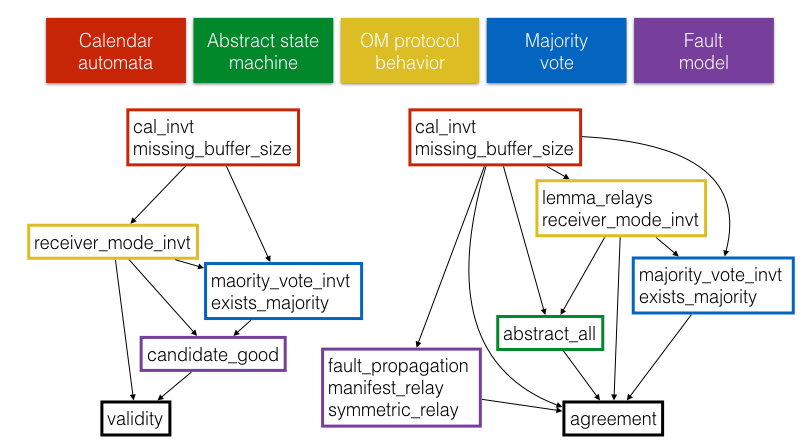
\includegraphics[width=\textwidth]{figs/proof-structure}
  \caption{Proof structure.}
  \label{fig:proof}
\end{figure}

The proof structure is shown in Figure~\ref{fig:proof}. The two graphs show the structure to prove validity and agreement, respectively. The nodes group related lemmas, and a directed edge from node $a$ to $b$ means lemmas of $b$ depend on $a$. For readability, we have replicated lemmas shared in the proofs of validity and agreement. Additionally, we have elided the dependencies between the lemmas within each node. The proofs are all $k=1$ inductive.

The lemmas are classified into five groups: calendar automata lemmas, abstract state machine lemmas, protocol behavior lemmas, majority vote lemmas, and fault model lemmas.

The calendar automata lemmas do not concern the system. The \emph{cal\_invt} lemma is a conjunction of basic properties about the calendar automata, essentially characterizing the axiomatization described in Section~\ref{sec:calendar}. Additionally, the \emph{missing\_buffer\_size} lemma relates the calendar to a node's message buffer: the messages received added to the empty messages equals the total number of possible messages to receive.

The \emph{abstract\_all} lemmas characterizes the transition between states of the abstract state machine. Technically, \emph{abstract\_all} also depends on ``boilerplate'' lemmas relating each state of the abstract state machine to a state variable representing it, which are elided for space.

The system itself includes both the lemmas characterizing the global protocol behavior as well as majority vote\lee{have we talked about the voting algorithm earlier?}. The global behavior concerns the entire distributed system, whereas the lemmas regarding the majority vote algorithm only concern the behavior of a single node. The proofs mechanize closely the proofs found in Boyer and Moore's original treatment~\cite{}.

Finally, the fault model lemmas relate the fault model to the system. The \emph{fault\_propagation} lemma connects the presence of faulty messages in the calendar with the fault status of nodes that receive those messages in subsequent rounds. The \emph{symmetric\_relay} and \emph{manifest\_relay} lemmas characterize the effect of symmetric and manifest faults, respectively, on the kinds of messages a receiver obtains from a faulty node. All the fault model lemmas mentioned so far are necessary for the agreement proof, but for validity, we need only \emph{candidate\_good}, proving that if the maximum fault assumption holds and the sender is nonfaulty, then no modified messages are received.

% ------------------------------------------------------------
\section{Experimental Results}\label{sec:experimental}

\lee{let's also check out scalability when we ``turn off'' faults. Also, how hard is it to turn them off or change the fault model? E.g., how many lines of spec need to be changed? Compare to rushby's?}

\begin{figure}
  \centering
  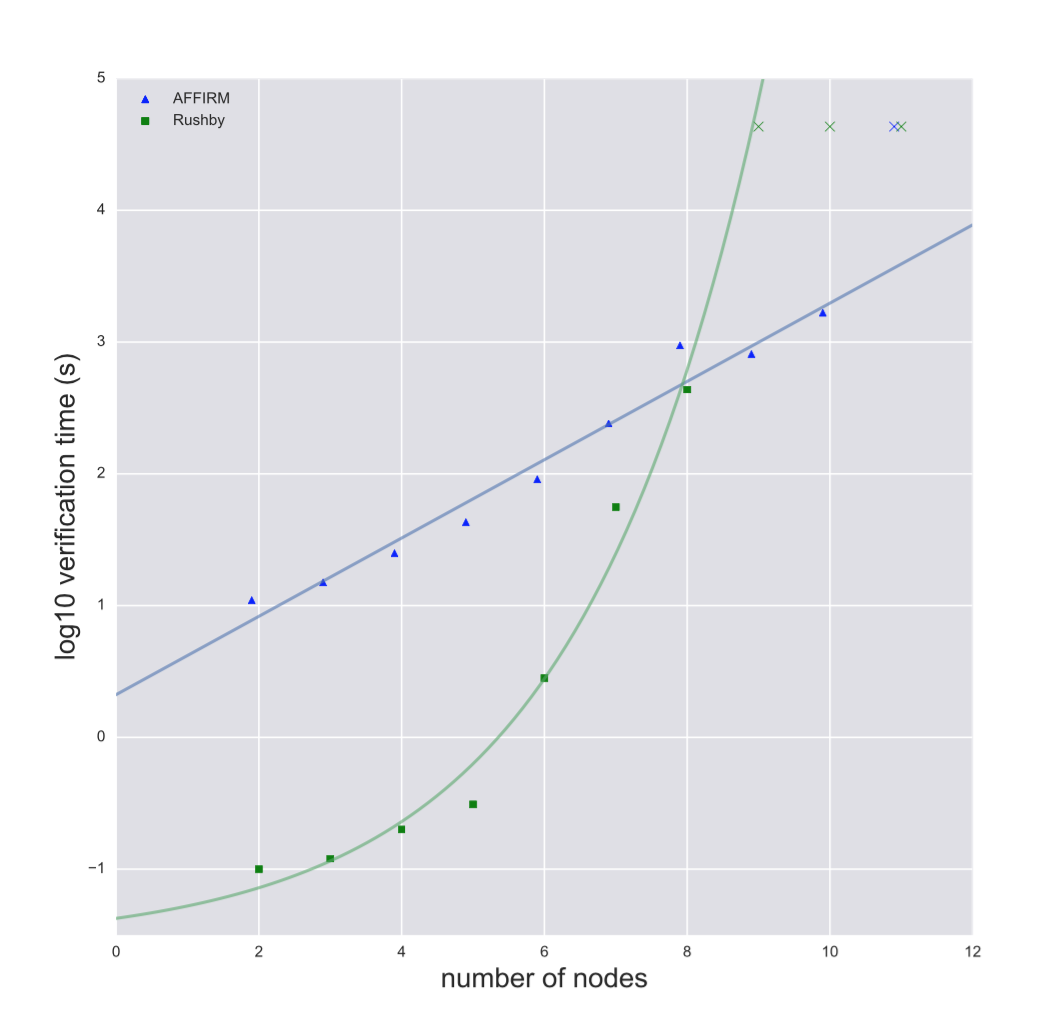
\includegraphics[width=8cm]{figs/benchmark}
  \caption{Comparison of number of nodes vs. verification time.}
  \label{fig:compare}
\end{figure}

% ------------------------------------------------------------
\section{Toward an Architectural Domain-Specific Language}\label{sec:adsl}

% ------------------------------------------------------------
\section{Related Work}\label{sec:related}
\lee{talk about om1 verification, comparing it to others.}

% ------------------------------------------------------------
\section{Conclusions}\label{sec:conclusions}

\bibliographystyle{IEEEtran}
\bibliography{paper}

\end{document}
